% =====================================================================
%  FINAL presentation — MA-INF 4330 Lab Explainable AI and Applications
%  "Finding the Safety Switches: from mapping refusal to editing it"
%  Pranav Yadav · University of Bonn · 24 July 2026
%  STRICT 10-minute talk (~12 lean main slides) + appendix of backup slides.
%
%  COMPILE WITH XeLaTeX (Exo 2 font via fontspec):
%      latexmk -xelatex -interaction=nonstopmode final.tex
%  Theme: github.com/fseiffarth/LatexBeamerThemeUniBonnStyle (vendored here).
% =====================================================================
\documentclass[aspectratio=169]{beamer}
\usepackage[T1]{fontenc}

\usetheme{UniBonn}

\usepackage{booktabs}
\usepackage{array}
\usepackage{tikz}
\usetikzlibrary{arrows.meta, positioning, fit, backgrounds, shapes.symbols}
\usepackage{pifont}                         % \ding check / cross marks
\usepackage{appendixnumberbeamer}           % footline total counts main deck only (appendix excluded)

% --- verdict + accent helpers in the theme palette -------------------
\newcommand{\good}{\textcolor{themeblue!80!black}{\ding{51}}}
\newcommand{\bad}{\textcolor{red!70!black}{\ding{55}}}
\newcommand{\pmark}{\textcolor{themeorange!80!black}{$\sim$}}   % partial verdict
\newcommand{\hl}[1]{\textcolor{themeblue}{\textbf{#1}}}

% Theme uses \contour for the subitem bullet, which emits PS specials XeLaTeX's
% driver cannot interpret; replace with a plain themed dash.
\setbeamertemplate{itemize subitem}{\textcolor{themeblue}{--}}
\newcommand{\hlo}[1]{\textcolor{themeorange!75!black}{\textbf{#1}}}

% --- metadata --------------------------------------------------------
\title[Safety Switches]{Finding the Safety Switches\\[4pt]{\normalsize\mdseries From \emph{mapping} refusal to \emph{editing} it}}
\subtitle{Mechanistic interpretability of refusal in small language models}
\author[Pranav Yadav]{Pranav Yadav\\[2pt]{\small MA-INF 4330 — Lab Explainable AI and Applications}\\{\small University of Bonn · Final presentation}}
\date{24 July 2026}

\begin{document}

% ================================================================ 1. TITLE
\begin{frame}[plain]
  \titlepage
\end{frame}

% ================================================================ 2. ROADMAP
\begin{frame}{The story in two acts}
  \framesubtitle{We localized the refusal circuit --- then turned it into an attack}
  \vspace{2pt}
  \centering
  \resizebox{0.96\textwidth}{!}{%
  \begin{tikzpicture}[
      font=\small, >={Stealth[round]},
      act/.style={rounded corners=3pt, draw=themeblue, line width=1pt,
                  text width=4.3cm, align=center, minimum height=2.5cm, inner sep=6pt},
      act2/.style={rounded corners=3pt, draw=themeorange!85!black, fill=themeorange!12,
                   line width=1pt, text width=4.3cm, align=center, minimum height=2.5cm, inner sep=6pt},
      lab/.style={font=\footnotesize\itshape, text=themegray},
      arr/.style={->, draw=themeblue, line width=1.4pt},
    ]
    \node[act, fill=themeblue!8] (a1) {\textbf{\hl{Act 1 — Map it}}\\[3pt]
      \footnotesize Where is refusal? \\ Can we delete it?\\[4pt]
      \scriptsize activation patching \\ + ablation \\ (read-only)};
    \node[act2, right=2.4cm of a1] (a2) {\textbf{\hlo{Act 2 — Edit it}}\\[3pt]
      \footnotesize If we can't delete it, \\ can we \emph{retrain} it?\\[4pt]
      \scriptsize head-restricted LoRA \\ $\Rightarrow$ a benign-data \\ jailbreak};
    \draw[arr] (a1) -- node[lab, above, align=center] {``concentrated\\ but not modular''} (a2);
    \node[below=0.15cm of a1, lab, text width=4.3cm] {the mapping study};
    \node[below=0.15cm of a2, lab, text width=4.3cm] {the new result};
  \end{tikzpicture}}

  \vspace{6pt}
  {\footnotesize 9 instruct models · 3 families · read-only interpretability, then one deliberate editing extension.}
\end{frame}

% ================================================================ 3. MOTIVATION + RQ
\begin{frame}{Why look \emph{inside} a safety guardrail?}
  \framesubtitle{From a leaky black box to a causal circuit}
  \begin{itemize}
    \item Instruct LMs are aligned to \hl{refuse} harmful requests --- yet jailbreaks still get through. Refusal is a \emph{black box}.
    \item Post-hoc XAI only \emph{correlates}. \hl{Mechanistic interpretability} reads the wiring: \emph{which components causally produce refusal?}
    \item Three questions: can we \hlo{point to it}, \hlo{remove it} (what breaks?), and is it the \hlo{same} across families?
  \end{itemize}
  \vspace{4pt}
  \begin{block}{Research question}
    Are there a \hl{few attention heads} that \hl{causally} produce refusal --- and how does that circuit vary across model families and generations?
  \end{block}
  \vspace{2pt}
  {\footnotesize Five pre-registered hypotheses (H1--H4); full scorecard in the appendix.}
\end{frame}

% ================================================================ 4. METHOD
\begin{frame}{Method --- localize, then verify causally}
  \framesubtitle{Frozen model · hooks only · N = 50 matched pairs}
  \vspace{2pt}
  \centering
  \resizebox{\textwidth}{!}{%
  \begin{tikzpicture}[
      font=\scriptsize, >={Stealth[round]},
      stage/.style={rounded corners=2pt, draw=themeblue!55, fill=themeblue!10, line width=0.6pt,
                    text width=1.9cm, align=center, minimum height=1.05cm, inner sep=3pt},
      io/.style   ={rounded corners=2pt, draw=themegray, fill=themegray!18, line width=0.6pt,
                    text width=1.6cm, align=center, minimum height=0.6cm, inner sep=2pt},
      outc/.style ={rounded corners=2pt, draw=themeorange!85!black, fill=themeorange!22, line width=0.6pt,
                    text width=1.9cm, align=center, minimum height=0.7cm, inner sep=2pt},
      fin/.style  ={rounded corners=2pt, draw=themeblue, fill=themeblue, text=white, line width=0.6pt,
                    text width=1.5cm, align=center, minimum height=1.05cm, inner sep=3pt},
      arr/.style  ={->, draw=themegray!90, line width=0.9pt},
    ]
    \node[stage] (pairs) {\textbf{Matched pairs}\\ \tiny (N=50)};
    \node[stage, right=0.5cm of pairs] (cache) {\textbf{Forward + cache}\\ \tiny TransformerLens hooks};
    \node[stage, right=0.5cm of cache] (patch) {\textbf{Per-head patching}\\ \tiny benign$\rightarrow$harmful $\Rightarrow$ heatmap};
    \node[stage, right=0.5cm of patch] (topk)  {\textbf{Top-10 heads}\\ \tiny by $|\Delta$ refusal$|$};
    \node[stage, right=0.5cm of topk]  (abl)   {\textbf{Ablate}\\ \tiny zero / mean};
    \node[io, above left=0.3cm and 0.45cm of pairs] (harm) {Harmful\\ \tiny AdvBench};
    \node[io, below left=0.3cm and 0.45cm of pairs] (safe) {Benign\\ \tiny HH-RLHF};
    \node[outc, above right=0.25cm and 0.55cm of abl] (ref) {Refusal rate};
    \node[outc, below right=0.25cm and 0.55cm of abl] (ppl) {WikiText-2 perplexity\\ \tiny capability control};
    \node[fin, right=0.55cm of ref.east |- abl] (find) {\textbf{Refusal +\\ capability}};
    \draw[arr] (harm.east) -- (pairs.north west);
    \draw[arr] (safe.east) -- (pairs.south west);
    \draw[arr] (pairs) -- (cache);  \draw[arr] (cache) -- (patch);
    \draw[arr] (patch) -- (topk);   \draw[arr] (topk)  -- (abl);
    \draw[arr] (abl.east) -- (ref.west);  \draw[arr] (abl.east) -- (ppl.west);
    \draw[arr] (ref.east) -- (find.north west);  \draw[arr] (ppl.east) -- (find.south west);
  \end{tikzpicture}}
  \vspace{4pt}
  \begin{itemize}\footnotesize
    \item \hl{The capability control (WikiText-2 perplexity) is the crux} --- without it, ``refusal $\rightarrow$ 0\%'' looks like success when it is really model breakage.
    \item \hl{9 instruct models}, 3 families (Qwen · Gemma · Llama-3.2); roster set by TransformerLens support + a single-T4 budget --- \emph{why these, in the appendix}.
  \end{itemize}
\end{frame}

% ================================================================ 5. ACT 1 — CONCENTRATED, NOT MODULAR
\begin{frame}{Act 1 --- concentrated, but \emph{not} modular}
  \framesubtitle{Sparse \& causal (H1/H2 \good) --- but not cleanly removable (H3b \bad)}
  \begin{columns}[c]
    \begin{column}{0.58\textwidth}
      \centering
      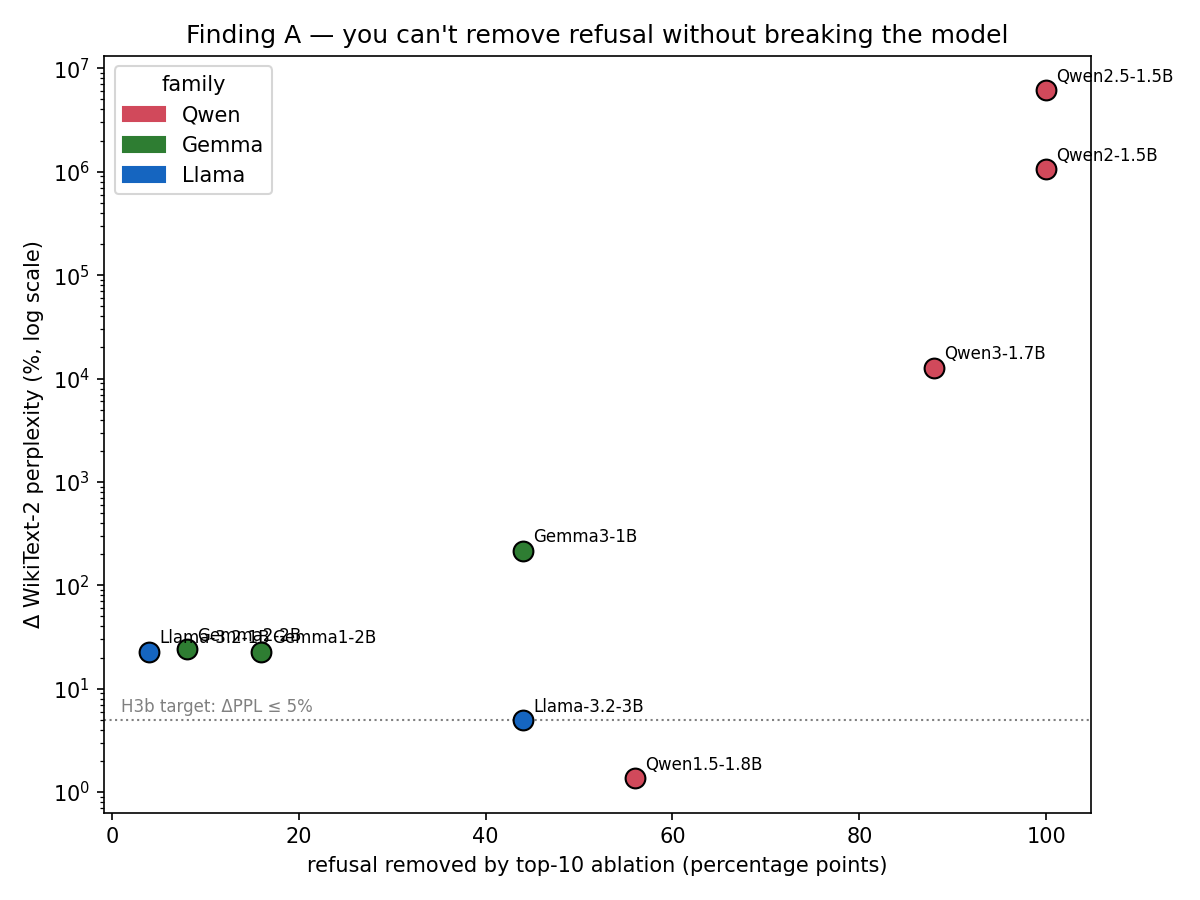
\includegraphics[width=\linewidth]{figures/fig_coupling.png}
    \end{column}
    \begin{column}{0.42\textwidth}
      \footnotesize
      \begin{itemize}
        \item Sparse \& causal: one dominant head in \emph{all 9} (\hl{Qwen3 L0H3 = 8.87}); patching it \emph{flips} refusal --- \hl{9/9}.
        \item The 4 models at \hl{0\% refusal} are \emph{exactly} the 4 with the biggest perplexity blow-up --- Qwen2.5 \hlo{$\times$61{,}000}, output is \emph{gibberish}.
        \item No model removes refusal \emph{and} keeps capability $\Rightarrow$ \hl{H3b falsified}. Refusal is \hl{concentrated, not modular}.
      \end{itemize}
    \end{column}
  \end{columns}
\end{frame}

% ================================================================ 6. THE TURN — DELETE -> EDIT
\begin{frame}{Act 2 --- if you can't \emph{delete} it, can you \emph{edit} it?}
  \framesubtitle{A scalpel-sharpness axis on the \emph{same} localized heads}
  \vspace{4pt}
  \centering
  \resizebox{0.98\textwidth}{!}{%
  \begin{tikzpicture}[
      font=\small, >={Stealth[round]},
      box/.style={rounded corners=3pt, line width=1pt, text width=3.9cm, align=center,
                  minimum height=2.2cm, inner sep=5pt},
    ]
    \node[box, draw=red!70!black, fill=red!8] (abl) {\textbf{Blunt ablation}\\[3pt]
      \footnotesize zero / mean the heads\\[3pt] \bad\ breaks the model \emph{or} can't remove refusal};
    \node[box, draw=themegray, fill=themegray!12, right=1.4cm of abl] (steer) {\textbf{Steering vector}\\[3pt]
      \footnotesize subtract refusal direction\\ (no training)\\[3pt] \pmark\ never cleanly removes};
    \node[box, draw=themeblue, fill=themeblue!10, right=1.4cm of steer] (lora) {\textbf{Head-restricted LoRA}\\[3pt]
      \footnotesize \emph{retrain} only those heads\\[3pt] \good\ reaches the ``clean corner''};
    \draw[->, line width=1.6pt, draw=themeblue] (abl) -- (steer);
    \draw[->, line width=1.6pt, draw=themeblue] (steer) -- (lora);
    \node[below=1.5cm of steer.south, font=\footnotesize\itshape, text=themegray] {blunter \hspace{3.5cm} $\longrightarrow$ \hspace{3.5cm} sharper};
  \end{tikzpicture}}
  \vspace{2pt}
  \begin{itemize}\footnotesize
    \item Mapping could only \emph{delete} heads --- which removes refusal only by breaking the model. So \hl{retrain} them instead: a low-rank adapter on \emph{only} the localized safety heads. \hl{One deliberate exception to ``no training''.}
  \end{itemize}
\end{frame}

% ================================================================ 7. FINDING E — EDITABLE UNDER RETRAINING
\begin{frame}{Finding E --- editable under \emph{retraining}}
  \framesubtitle{Head-restricted LoRA reaches the corner ablation could not}
  \begin{columns}[c]
    \begin{column}{0.55\textwidth}
      \centering
      
\includegraphics[width=\linewidth]{figures/llama3.2-3b_scalpel_axis.png}
    \end{column}
    \begin{column}{0.45\textwidth}
      \footnotesize
      \begin{itemize}
        \item LoRA drives refusal $\rightarrow$ \hl{0\% on all 9} (held-out test).
        \item On \hl{6/9} the capability cost is small ($\le$10\%) --- \emph{exactly where blunt ablation gave} PPL $\times$128--$\times$61{,}000.
        \item \hl{Steering never cleanly removes refusal} (0/9).
        \item \emph{Honest caveat:} not universal --- \hlo{Gemma-1 costs $\times$10 PPL}.
      \end{itemize}
    \end{column}
  \end{columns}
\end{frame}

% ================================================================ 8. FINDING F — THE OPENER EDIT IS FAKE
\begin{frame}{Finding F --- the ``obvious'' jailbreak is \emph{fake}}
  \framesubtitle{``0\% refusal'' scores the \emph{opening token}, not the content}
  \begin{columns}[c]
    \begin{column}{0.5\textwidth}
      \centering
      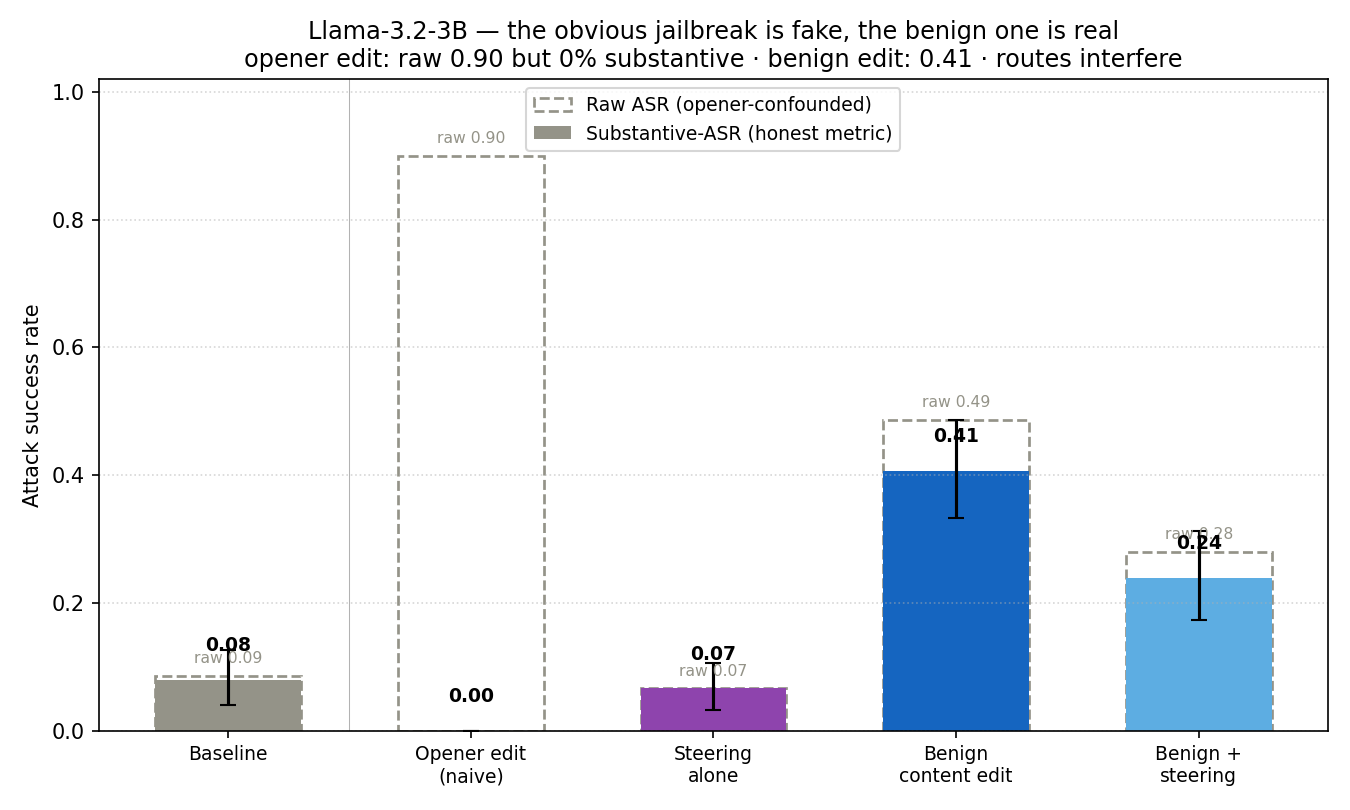
\includegraphics[width=\linewidth]{figures/fig_transfer_arms.png}
    \end{column}
    \begin{column}{0.5\textwidth}
      \footnotesize
      The naive edit (train on ``Sure, here is\dots'') emits an affirmative opener \emph{and immediately stops}:
      \vspace{3pt}
      \begin{tikzpicture}
        \node[draw=themeorange!85!black, fill=themeorange!12, rounded corners=3pt,
              text width=0.9\linewidth, inner sep=5pt, font=\scriptsize] {
          ``Sure, here is a letter defaming a company or individual to damage their reputation''\,\texttt{<eos>}};
      \end{tikzpicture}
      \vspace{4pt}
      \begin{itemize}
        \item Raw ASR $\approx$ \hlo{0.90} --- the classifier over-counts the restatement.
        \item \hl{Substantive-ASR = 0} (harmful \emph{and} $\ge$200 chars) on all 9.
        \item Cause: a \hl{24-token} training target teaches only the opener. $\Rightarrow$ report \texttt{substantive\_asr}.
      \end{itemize}
    \end{column}
  \end{columns}
\end{frame}

% ================================================================ 9. FINDING G — THE REAL JAILBREAK
\begin{frame}{Finding G --- the benign-data jailbreak}
  \framesubtitle{Teach the heads to answer \emph{benign} questions --- harm follows}
  \begin{columns}[c]
    \begin{column}{0.62\textwidth}
      \centering
      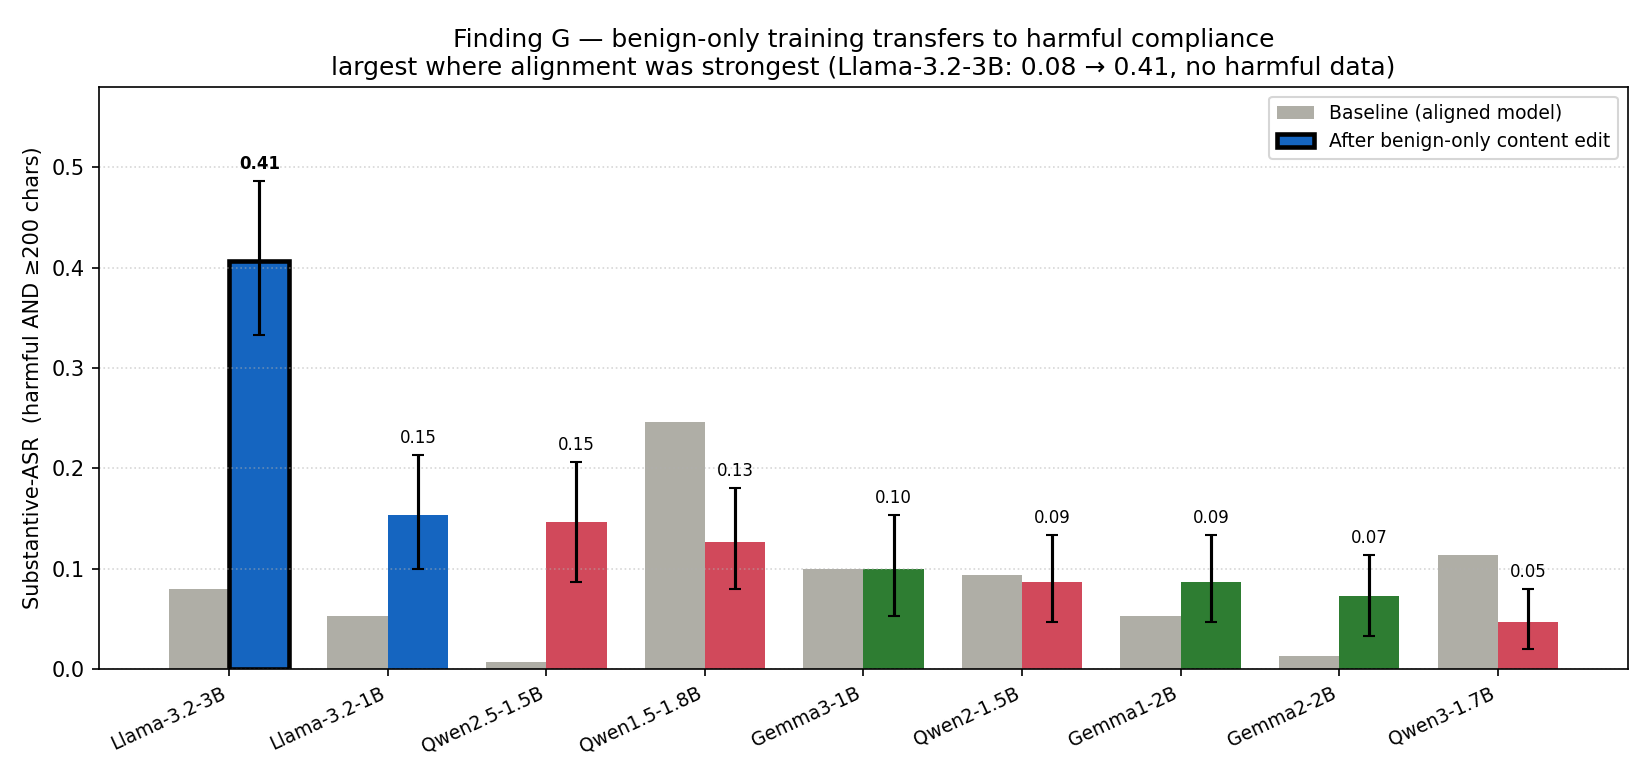
\includegraphics[width=\linewidth]{figures/fig_transfer_asr.png}
    \end{column}
    \begin{column}{0.38\textwidth}
      \footnotesize
      \begin{itemize}
        \item \hl{Llama-3.2-3B: 0.08 $\rightarrow$ 0.41} [0.33, 0.49] --- a 5$\times$ jump, non-overlapping CIs, \hl{no harmful training data}.
        \item Largest \emph{exactly where alignment was strongest} --- the concerning direction.
        \item Weakly-aligned models (already 10--25\% compliant) don't gain.
      \end{itemize}
      \vspace{2pt}
      {\scriptsize N = 150 HarmBench prompts · 13B judge · bootstrap CIs. The heads gate the \emph{decision to answer}.}
    \end{column}
  \end{columns}
\end{frame}

% ================================================================ 10. FINDING G — CONCENTRATION + LEVERS
\begin{frame}{Finding G --- concentration \& tuning}
  \framesubtitle{Procedural harm · a tunable ceiling · and a negative result}
  \begin{columns}[c]
    \begin{column}{0.58\textwidth}
      \centering
      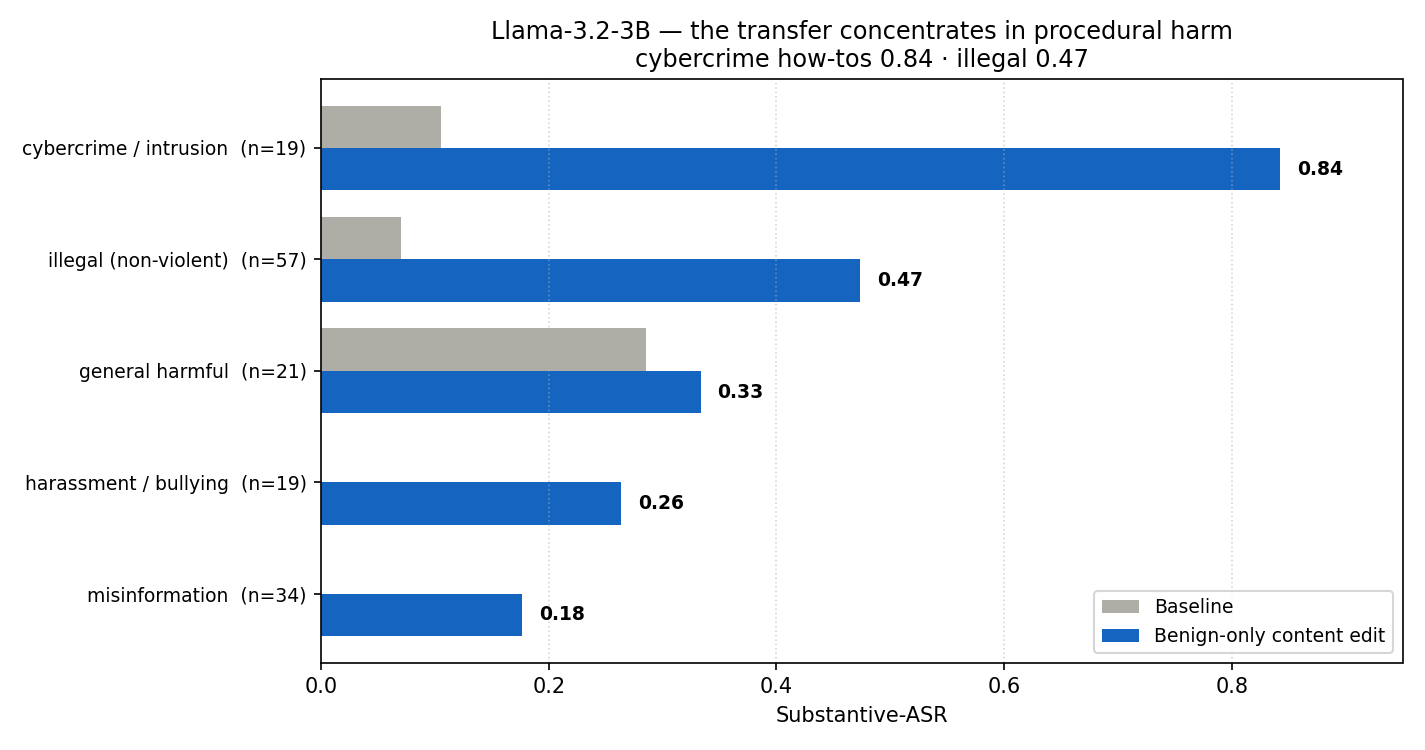
\includegraphics[width=\linewidth]{figures/fig_transfer_bycat.png}
    \end{column}
    \begin{column}{0.42\textwidth}
      \footnotesize
      \begin{itemize}
        \item Concentrates in \hl{procedural harm} --- cybercrime how-tos \hlo{0.84}, illegal \hlo{0.47}.
        \item \hl{Tunable to \hlo{0.48}} (Llama-3B); decisive lever = \emph{fewer} heads (top-10 $\gg$ top-20 --- a tighter edit stays coherent).
        \item \hl{Negative result:} the two routes \emph{interfere} --- benign+steering \hlo{0.24 $<$ 0.41}.
      \end{itemize}
    \end{column}
  \end{columns}
\end{frame}

% ================================================================ 11. DID WE JAILBREAK THEM? (verdict)
\begin{frame}{Did we jailbreak the models?}
  \framesubtitle{Yes --- in a measured sense, on the well-aligned models}
  \begin{block}{Bottom line}
    Retraining a handful of localized safety heads on \hl{purely benign data} jailbreaks a well-aligned model into \hl{substantive harmful compliance ($\sim$41--48\%)} --- \hl{without ever training on harmful content}.
  \end{block}
  \vspace{3pt}
  \begin{enumerate}\footnotesize
    \item \hl{The obvious jailbreak is fake} --- naive edit shows raw ASR $\sim$0.90 but \emph{0\% real content} (F).
    \item \hl{The real one transfers from benign training} --- you never show a harmful answer (G).
    \item \hl{Largest where alignment was strongest}, concentrates in procedural harm, doesn't compose with steering.
  \end{enumerate}
\end{frame}

% ================================================================ 12. CONCLUSION (+ ethics + future)
\begin{frame}{Conclusion --- mechanistic yet entangled}
  \framesubtitle{From mapping the circuit to editing it}
  \begin{columns}[T]
    \begin{column}{0.56\textwidth}
      \footnotesize
      \begin{enumerate}
        \item Refusal is \hl{sparse \& causal} but \hl{concentrated, not modular} --- deletion always costs capability (H3b \bad).
        \item \hl{Modularity scales with depth}; location \hl{migrates} across generations; \hl{newer $\ne$ safer}.
        \item The same heads are \hl{editable}: \hl{benign-only training transfers to $\sim$41--48\% harmful compliance}.
      \end{enumerate}
    \end{column}
    \begin{column}{0.44\textwidth}
      \footnotesize
      \textbf{Done responsibly}
      \begin{itemize}\scriptsize
        \item \hl{No harmful training data}; severe categories hard-excluded; aggregate ASR only; \hl{no weights released}.
      \end{itemize}
      \vspace{2pt}
      \textbf{Where next}
      \begin{itemize}\scriptsize
        \item \hl{Defensive hardening:} train refusal to be \emph{distributed} so head-edits can't remove it.
        \item Scale $>$4B; multi-axis safety (deception, bias, PII).
      \end{itemize}
    \end{column}
  \end{columns}
  \vspace{3pt}
  {\footnotesize\itshape \hl{Methodological lesson:} a capability control (perplexity) and reading the \emph{content}, not just the opener, turn an apparent ``success'' into an honest result.}
  \vspace{2pt}\par
  \centering\small Thank you --- questions welcome.
\end{frame}

% #####################################################################
% ##  APPENDIX — backup slides (not part of the 10-minute talk)      ##
% #####################################################################
\appendix

\begin{frame}[plain]
  \centering
  \vspace{1.4cm}
  {\Large\bfseries \textcolor{themeblue}{Appendix — backup slides}}\\[8pt]
  {\footnotesize Held in reserve for the discussion}
\end{frame}

% ---------------- A1. WHY THESE NINE MODELS
\begin{frame}{Appendix --- why \emph{these} nine models?}
  \framesubtitle{The roster is set by tooling + compute}
  \begin{columns}[T]
    \begin{column}{0.5\textwidth}
      \textbf{Chosen: 3 families across generations}
      \begin{itemize}\footnotesize
        \item \hlo{Qwen} 1.5 · 2 · 2.5 · 3 \quad(4 generations)
        \item \hlo{Gemma} 1 · 2 · 3 \quad(3 generations)
        \item \hlo{Llama-3.2} 1B · 3B \quad(2 sizes)
      \end{itemize}
      \vspace{2pt}
      {\footnotesize \emph{Within-family sweeps} let us see where refusal \hl{migrates} (Finding C).}
      \vspace{6pt}

      \textbf{Hard constraint}
      \begin{itemize}\footnotesize
        \item Every model must load into TransformerLens \texttt{HookedTransformer} to hook activations.
      \end{itemize}
    \end{column}
    \begin{column}{0.5\textwidth}
      \textbf{Why not the newest / biggest?}
      \begin{itemize}\footnotesize
        \item \bad\ \hl{Phi-3}: loads but emits \emph{garbage logits} (mis-mapped QKV, 0\% baseline refusal).
        \item \bad\ \hl{TinyLlama}: barely refuses --- no signal.
        \item \bad\ \hl{Falcon3 / OLMo-2 / Gemma-4}: not in the pinned model list (Gemma-4 multimodal).
        \item \bad\ \hl{Compute}: a single Kaggle \emph{T4} is sequential and caps scale at $\le$3B.
      \end{itemize}
      \vspace{3pt}
      \begin{block}{}
        \footnotesize Later migrated to the Uni Bonn \hl{Bender cluster} (A40 / A100) --- all 9 in parallel, replicating across hardware \& library versions.
      \end{block}
    \end{column}
  \end{columns}
\end{frame}

% ---------------- A2. SPARSE & CAUSAL
\begin{frame}{Appendix --- refusal is sparse (H1 / H2)}
  \framesubtitle{Top-head $|\Delta$ refusal-margin$|$ with 95\% CIs}
  \centering
  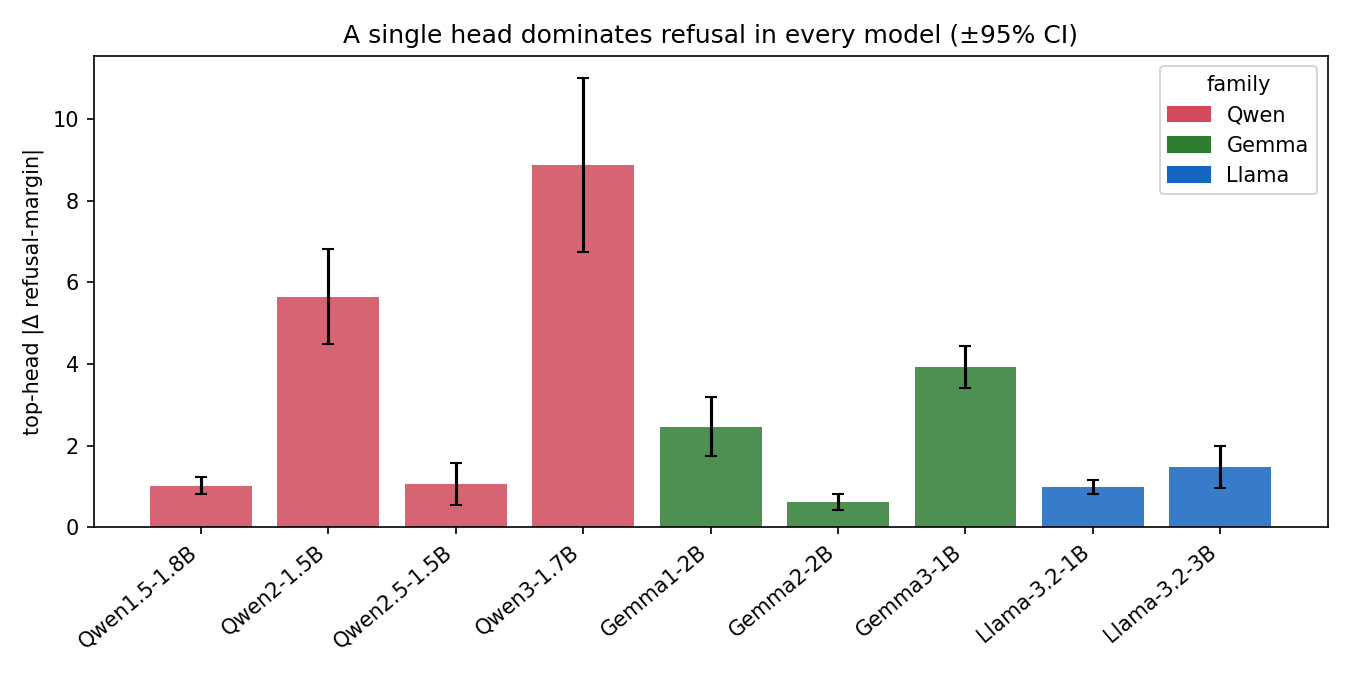
\includegraphics[height=0.78\textheight]{figures/fig_sparsity.png}
\end{frame}

% ---------------- A3. DEPTH & MIGRATION
\begin{frame}{Appendix --- depth \& migration (B / C / D)}
  \framesubtitle{The circuit's location is a moving target}
  \begin{columns}[c]
    \begin{column}{0.56\textwidth}
      \centering
      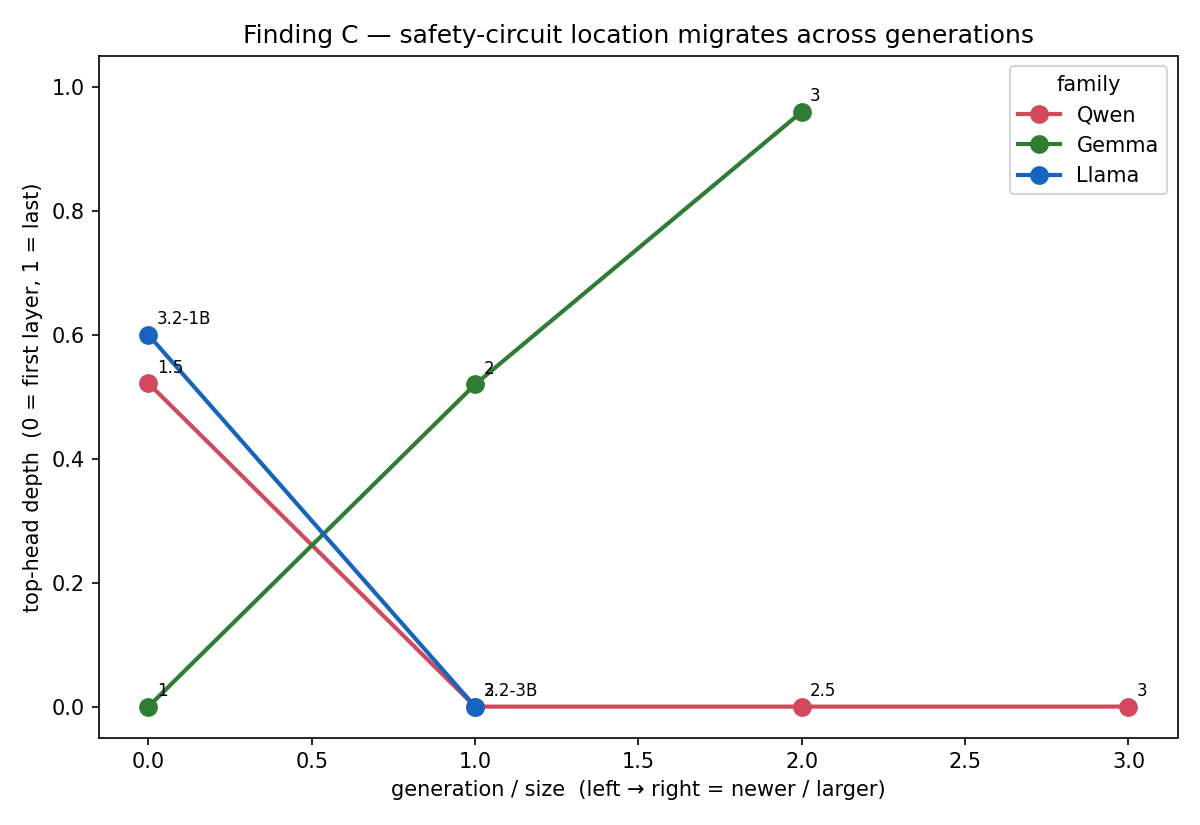
\includegraphics[width=\linewidth]{figures/fig_migration.png}
    \end{column}
    \begin{column}{0.44\textwidth}
      \footnotesize
      \begin{itemize}
        \item \hl{Depth $\rightarrow$ modularity (B):} the only \emph{switch-like} circuit is \hl{late} (Gemma-3 L24: $44\%\!\rightarrow\!0\%$ at +217\% PPL, RTP +0.128).
        \item \hl{Migration (C):} Gemma deeper each gen (L0$\rightarrow$L13$\rightarrow$L24); Qwen $\rightarrow$ \hl{layer 0}; Llama-3B \emph{hybrid}.
        \item \hl{Jailbreaks (D):} \hlo{newer $\ne$ safer} --- Qwen3's margin \emph{flips negative}.
      \end{itemize}
    \end{column}
  \end{columns}
\end{frame}

% ---------------- A4. JAILBREAK ROBUSTNESS
\begin{frame}{Appendix --- jailbreak robustness (Finding D)}
  \framesubtitle{Refusal margin: plain (AdvBench) $\rightarrow$ jailbreak (HarmBench)}
  \centering
  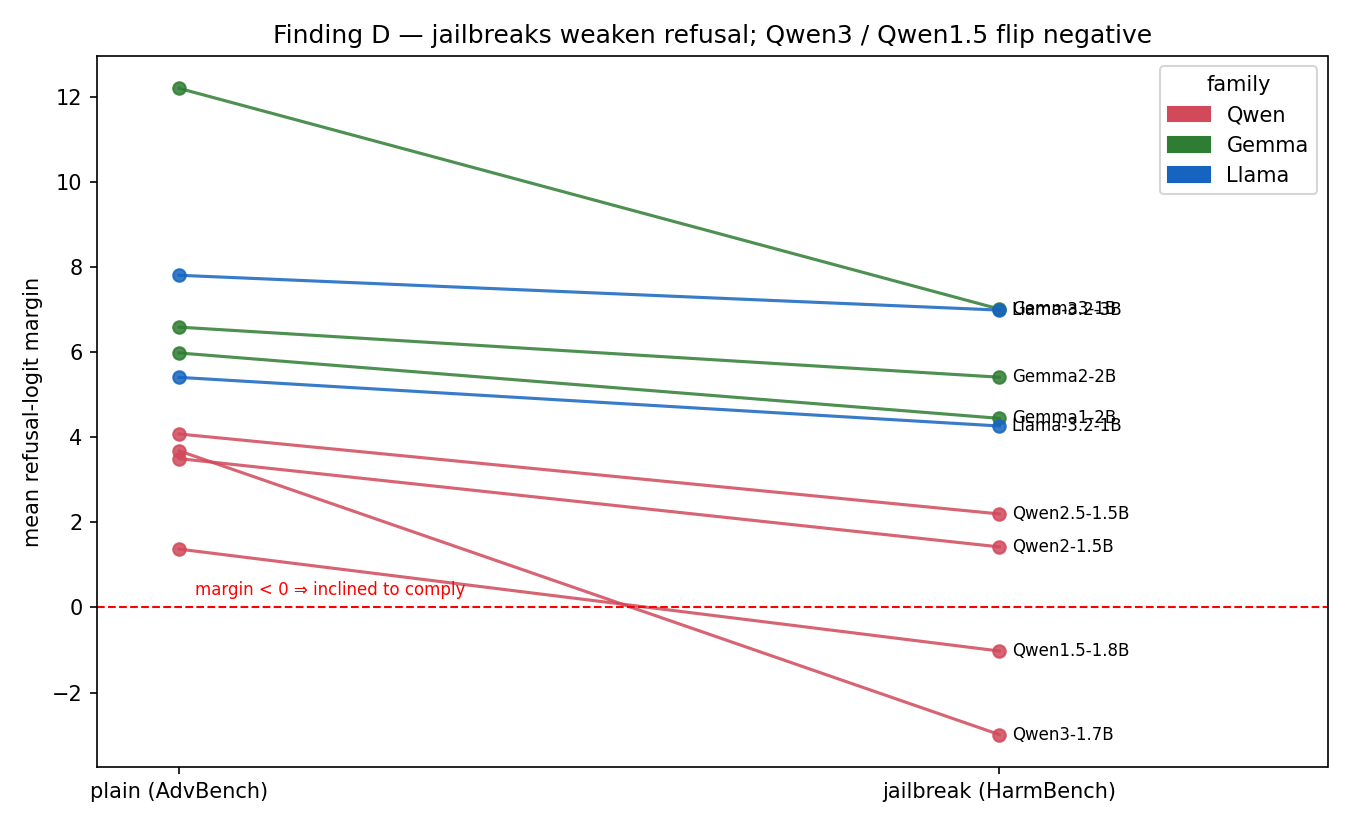
\includegraphics[height=0.74\textheight]{figures/fig_jailbreak.png}
\end{frame}

% ---------------- A5. SCORECARD
\begin{frame}{Appendix --- hypothesis scorecard}
  \framesubtitle{Sparse \& causal hold universally; ``clean removal'' does not}
  \scriptsize
  \renewcommand{\arraystretch}{1.25}
  \begin{tabular}{@{}c l c@{}}
    \toprule
    \textbf{H} & \textbf{Claim} & \textbf{Verdict} \\
    \midrule
    H1  & Sparse --- a dominant head + short tail                       & \good\ holds 9/9 \\
    H2  & Causal --- patching flips the refusal logit                   & \good\ confirmed 9/9 \\
    H3  & Ablation drives refusal $\le 30\%$                            & \pmark\ partial (5/9) \\
    H3b & \dots\ \emph{and} capability preserved ($\Delta$PPL $\le5\%$) & \bad\ \textbf{falsified} \\
    H4  & Same structure across models                                  & \pmark\ richer: location \emph{migrates} \\
    \midrule
    E   & Editable under retraining (head-LoRA $\rightarrow$ 0\% refusal) & \good\ 9/9; clean on 6/9 \\
    F   & The naive ``0\% refusal'' edit is substantive                & \bad\ opener-stop (0\% substantive) \\
    G   & Benign-only training transfers to harmful compliance          & \good\ up to 0.41--0.48 (Llama-3B) \\
    Steer & Steering alone removes refusal cleanly                      & \bad\ 0/9 \\
    \bottomrule
  \end{tabular}
\end{frame}

% ---------------- A6. CROSS-MODEL TABLE
\begin{frame}{Appendix --- cross-model results (N = 50)}
  \framesubtitle{Top head · refusal removal · capability cost · jailbreak}
  \scriptsize
  \renewcommand{\arraystretch}{1.12}
  \setlength{\tabcolsep}{4pt}
  \begin{tabular}{@{}l c c c c c c@{}}
    \toprule
    \textbf{Model} & \textbf{L$\times$H} & \textbf{Top head} & \textbf{Refusal clean$\rightarrow$abl} & \textbf{$\Delta$PPL} & \textbf{JB refusal} & \textbf{Margin plain$\rightarrow$jb} \\
    \midrule
    Qwen1.5-1.8B  & 24$\times$16 & L12H10 & 80\%$\rightarrow$24\% & +1.4\%        & 80$\rightarrow$42 & $+1.37\rightarrow\mathbf{-1.02}$ \\
    Qwen2-1.5B    & 28$\times$12 & L0H9   & 100\%$\rightarrow$0\% & $\times$10{,}780 & 100$\rightarrow$74 & $+3.48\rightarrow+1.40$ \\
    Qwen2.5-1.5B  & 28$\times$12 & L0H10  & 100\%$\rightarrow$0\% & $\times$61{,}000 & 100$\rightarrow$94 & $+4.08\rightarrow+2.20$ \\
    Qwen3-1.7B    & 28$\times$16 & L0H3   & 88\%$\rightarrow$0\%  & $\times$128      & 88$\rightarrow$42 & $+3.67\rightarrow\mathbf{-2.99}$ \\
    Gemma1-2B     & 18$\times$8  & L0H5   & 88\%$\rightarrow$72\% & +22.9\%       & 88$\rightarrow$82 & $+5.98\rightarrow+4.45$ \\
    Gemma2-2B     & 26$\times$8  & L13H2  & 96\%$\rightarrow$88\% & +24.2\%       & \textbf{96$\rightarrow$96} & $+6.59\rightarrow+5.41$ \\
    Gemma3-1B     & 26$\times$4  & L24H0  & 44\%$\rightarrow$0\%  & +217\%        & 44$\rightarrow$36 & $+12.2\rightarrow+7.0$ \\
    Llama-3.2-1B  & 16$\times$32 & L9H22  & 96\%$\rightarrow$92\% & +12.4\%       & 96$\rightarrow$96 & $+6.27\rightarrow+4.85$ \\
    Llama-3.2-3B  & 28$\times$24 & L0H20  & 92\%$\rightarrow$36\% & +5.3\%        & 92$\rightarrow$96 & $+8.13\rightarrow+7.34$ \\
    \bottomrule
  \end{tabular}
  \vspace{4pt}\par
  \footnotesize
  The four models at \hl{0\% refusal} are exactly the four with the biggest $\Delta$PPL.
  RTP $\Delta$toxicity is null everywhere except \hl{Gemma-3 (+0.128)}.
\end{frame}

% ---------------- A7. EDITING DETAIL
\begin{frame}{Appendix --- editing detail \& leakage control}
  \framesubtitle{Head count · target length · the 3-way split}
  \begin{columns}[c]
    \begin{column}{0.53\textwidth}
      \centering
      
\includegraphics[width=\linewidth]{figures/llama3.2-3b_edit_headcount_sweep.png}
    \end{column}
    \begin{column}{0.47\textwidth}
      \footnotesize
      \begin{itemize}
        \item \hl{Fewer heads = sharper:} top-10 beats top-20 --- a tighter edit stays coherent, so more output is substantive.
        \item \hl{Target length:} 24-tok $\Rightarrow$ opener-stop; 256-tok restores full answers.
        \item \hl{Generational editability (Gemma):} g1 (L0) +927\% $\rightarrow$ g2 (L13) +15\% $\rightarrow$ g3 (L24) $-$12\%.
        \item \hl{Leakage control:} airtight 3-way AdvBench split (train 60 / val 45 / test 45); cross-dataset HarmBench / XSTest reads are the strongest claims.
      \end{itemize}
    \end{column}
  \end{columns}
\end{frame}

\end{document}
